\section{Modeling of Giraf administration}
To understand how user, children and applications will be represented and connected in the system, a model  has been made with only the more important classes included. This model is in Figure \vref{fig:classOversigt}. The application we are creating is called \textit{Giraf Administration} which then would have one user and many applications. As shown in the figure the "User" would either be a \textit{Parent} or a \textit{Kindergarten teacher}. In the model the user has a connection with a child, who also has a connection to its \textit{Child's mobile device}.

In reality it is possible for the child to have more than one device and that has been taken into account. This also means that there is an indirect connection between the \textit{User} and \textit{Child's mobile device} that has "\textit{Giraf mobile application} installed, which should be administered by the \textit{user} through the \textit{Giraf administration}. That means, that to administer the mobile application, the \textit{user}'s \textit{Giraf administration} must have a corresponding version of \textit{Giraf application administration}. However, some of the \textit{Giraf administration applications} do not have a mobile version which makes them a \textit{User application}. This is all represented in the model in Figure \vref{fig:classOversigt}.


\begin{figure}[!ht]
	\centering
		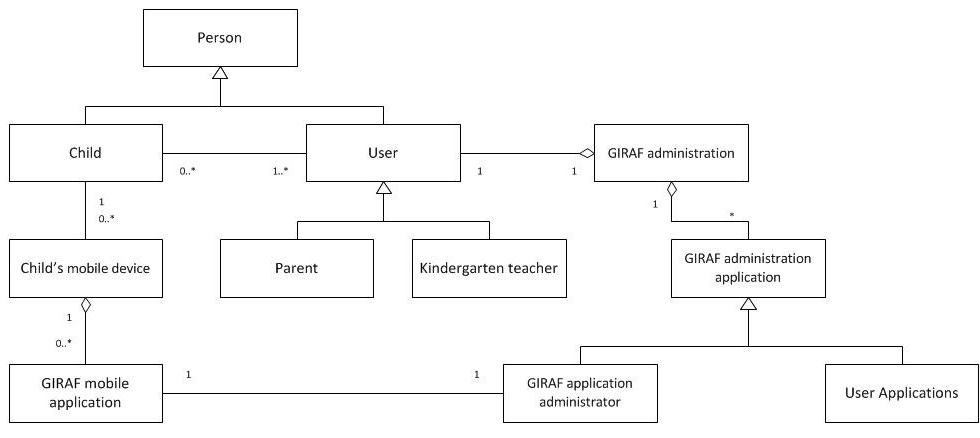
\includegraphics[width=1.00\textwidth]{img/classOversigt.jpg}
	\caption{Giraf administration program}
	\label{fig:classOversigt}
\end{figure}
\newpage